\section{Background}\label{sec:background}
\label{sec:cast}

In this section, we define the terms needed to state Gauss-Bonnet theorem.
We then present a proof of the theorem for a discrete surfaces.


\subsection{Continuous Curvature}


At a point on a parametrized curve  in $\RR^3$,
how should we quantify the curvature?
A straight line should have zero curvature and the curvature of the unit circle ought to be one.
We would also like a way to differentiate
between turning left and turning right, that is we want curvature to be a signed quantity.

One way to think curvature is to approximate the curve at a point with a circle,
then define the curvature to be the inverse of the radius of this circle $k=\frac{1}{r}$.
Such a circle is called the \EMPH{osculating circle}.
See \figref{osculating-circle} for an example.
For a straight line the curvature is zero, 
every point on the unit circle has curvature one 
and we can distinguish between
which way we are turning by which side of the curve the osculating circle is on,
 and as we hoped.
 This osculating-circle idea can be extend
to  surfaces in $\R^3$, by considering the \EMPH{osculating sphere},
 the sphere that best approximates the surface at a point.
However, for saddle points on a surface it is not clear which sphere
best approximates the surface. Moreover, we would like a formula to compute the curvature.

A curve $\gamma(t)$ in $\RR^3$ is \EMPH{smooth} on an open interval $I$
if $\gamma'$ is continuous and $\gamma'(t)\neq 0$ on $I$. 
If $\gamma$ is smooth it has a well-defined unit tangent vector $T(t)=\frac{\gamma'(t)}{|\gamma'(t)|}.$
The \EMPH{curvature} at a point is the magnitude of the rate of change of the unit tangent vector with 
respect to arc length

\begin{equation} \label{eqn:kappa}
\kappa=\bigg  | \frac{T'(t)}{\gamma'(t)}\bigg |.
\end{equation}
where $s$ is arc length.

For example, take a circle of radius $r$, parameterized by $C(t)=\left(r\cos(t),r\sin(t)\right)$.
We have $\frac{dC}{dt}=C'(t)=\left(-r\sin(t),r\cos(t)\right)$ and $|C'(t)|=r$.
Then $T(t)=\left(-\sin(t),\cos(t)\right)$ and $T'(t)=\left(-\cos(t),-\sin(t)\right)$.
So, $\kappa(t)=\frac{1}{r}$ and our definition of curvature agrees with the
osculating circle intuition above. 
\eqnref{kappa} can be rewritten in the following more computational friendly form 
\begin{equation} \label{eqn:kappa1}
\kappa(t)=\frac{|\gamma'(t)\times \gamma''(t)|}{|\gamma'(t)|^3}.
\end{equation}

Since we traverse $\gamma$
at unit speed, $\gamma'(t)^2=1,$ and by the chain rule, $\gamma'\cdot \gamma''=0,$
so  the second derivative is orthogonal to $\gamma'$. Thus, the
vector $\gamma''=N$ is normal to the $\gamma$. 
By taking the cross product of $N$ and $T$ we obtain a vector $B$.
The vectors $T,N$ and $B$ form the \emph{Fernet frame} of $\gamma$ a $p.$

Now we consider the curvature of a point on a surface. In one dimension we are
able parameterize our curve. Similarly, we require the ability to parameterize a surface.
A \EMPH{parameterized surface} is a map $\phi:U\subset \RR^2 \to \RR^3$ that
is differentiable. The set $\phi(U)\subset \RR^3$ is called the \EMPH{trace} of $\phi$.
If the differential $d\phi_q:\RR^2\to \RR^3$ is one-to-one for all $q\in U$ then
we say $\phi$ is \EMPH{regular}. In other words, let $(u,v)$ be coordinates of $U\subset \RR^2,$
a surface is regular if $\frac{\partial\phi}{\partial u}$
and $\frac{\partial\phi}{\partial v}$ are linearly independent for all $q\in U$.

Let $S$ be a regular surface, then at each point $p\in S$ the set of tangent vectors
to parameterized curves in $S$ through $p$ forms a plane.
A \EMPH{tangent vector} to $S$ at $p$ is a map $\xi:(-\epsilon,\epsilon)\to S$ with $\xi(0)=p$.
The set of all tangent vectors is the \EMPH{tangent plane} and it corresponds to the image
of the differential map $d\phi_q(\RR^2)\subset \RR^3$ (prop. 1 \cite{doc76}).
Let $S_1$ and $S_2$ be two surfaces with $\sigma:V\subset S_1\to S_2$ a differentiable map.
At $p\in S_1$ the map $d\sigma_p:T_p(S_1)\to T_{\sigma(p)}(S_2)$ is called the
\EMPH{differential} of $\sigma$ at $p$.

By choosing two linearly independent paths through $p\in S$ we can obtain the explicit tangent
plane and define a normal vector $N$ at $p$.
Every plane containing the normal vector will intersect the surface.
The intersection of the surface and each normal plane is a curve in $\RR^3$. 
Let $\kappa_1$ denote the maximum curvature over all normal planes
and let $\kappa_2$ denote the minimum curvature over all normal planes.
The \EMPH{Gaussian curvature} of a point on a surface is
$K=\kappa_1\kappa_2.$

There are several equivalent ways to calculate curvature of a surface.
Once we choose a chart we define a clockwise orientation. If the clockwise
orientation can be consistently extended to the entire surface, we say
the surface is \EMPH{orientable}.
For an orientable surface $S$, the map that  $N:S\to \Sp^2$ that sends each
normal in $S$ to the corresponding point on $\Sp^2$ is
the \EMPH{Gauss map}.
The derivative of the Gauss map, $dN(p)$ quantifies the rate of change of
the normal vector ($dN$ is often called the \emph{Weingarten map} \cite{Crane:2013}).
Thus, $dN_p:T_p(S)\to T_{N(p)}(\Sp^2)$, but since $T_p(S)$ and $T_{N(p)}(\Sp^2)$
are parallel we can define $dN_p$ to be a linear map on $T_p(S)$.
Remarkably, the determinant of $dN(p)$ is equal to the Gaussian curvature.


We will consider one-dimensional curves that are the boundary of two-dimensional
surfaces in $\R^3.$ Let $\gamma$ denote such a curve parametrized by arc length.
In a surface, a \EMPH{geodesic} is a curve that is a shortest path
between two points in the surface. 
For example, on $\Sp^2$, the equator is a geodesic
and an inhabitant would view a geodesic as a straight line. 
The \EMPH{geodesic curvature} quantifies how close $\gamma$ is to being a geodesic.
Geodesics have zero geodesic curvature. 
For a formal definition see \cite{doc76}.







\subsection{The Discrete Gauss-Bonnet}

Discrete curvature is an oxymoron. In a triangulated surface,
the curvature is zero or we are on a vertex where tangent vectors are not defined.
One application of the Gauss-Bonnet Theorem will be to confirm that the definition of discrete curvature 
given below is reasonable.
We would like our definition of discrete curvature to agree with
our intuition, that is if two segments co-linear, the curvature should be zero
and the curvature should signed.

Consider a triangulated regular surface $S$ with boundary $\partial(S)$.
The boundary is a one dimensional piecewise linear curve in $\R^3.$
As with simple polygons in the plane, at each vertex $v\in \partial(S)$ 
we have an exterior angle and a complementary interior angle.
The exterior angle has the desired properties of a curvature definition mentioned above.
The interior angle might consist of many triangles.
Let $F_v$  denote the set of faces incident to $v$ and let
$\alpha_f$ denote the angle in face $f$ at $v$.
The \EMPH{discrete geodesic curvature}
of $v$  is
$$k_{g}(v)= \pi-\sum_{f\in F_v}\alpha_f.$$
Notice that if $v$ lies on a straight line, then $\sum_{i}\alpha_f=\pi$
and the curvature is zero as we would expect.
The word geodesic is used because we are measuring how close
a curve is to being straight with respect to the surface we are on.


A geometric definition of discrete Gaussian curvature is the following:
\begin{definition}[Discrete Gaussian curvature]\label{def:discrete-curvature-vertex}

The discrete \EMPH{Gaussian curvature} at a vertex $v$ is the area on the unit 
sphere bounded by a spherical polygon whose vertices are the unit normals of 
the faces around $v$.

\end{definition}

If a vertex is on a flat surface, then the unit normals are all pointed
in the same direction and the Gaussian curvature is zero.

\begin{figure}[htb]
\centering
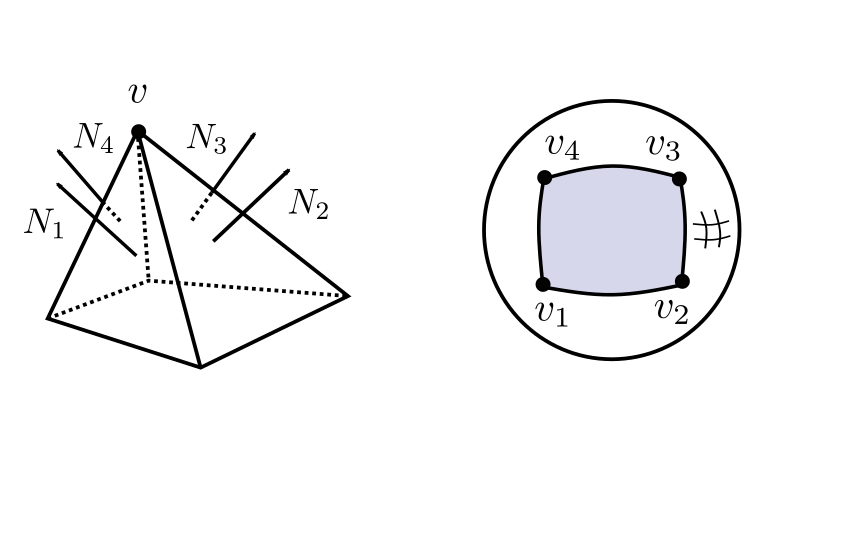
\includegraphics[width=.5\textwidth]{curvature/discrete-curvature}
\caption{Consider the vertex $v$ in the figure on the left. The curvature of $v$
is the area on the sphere shown on the right. We rotated the sphere
in order to see the entire polygon.}
\label{fig:discrete-curvature}
\end{figure}


Let $\alpha_i$ denote the angle of a triangle incident to $v$, 
we next show that the interior angle of the polygon $\beta_i$ on the 
sphere is supplementary $\alpha_i$.

\begin{equation} \label{eqn:switcheroo}
\beta=\pi-\alpha.
\end{equation}
Notice that the edge between two faces
on a triangulated surface
is perpendicular to the normal vectors of the faces.
So, the line connecting two normal vectors will intersect the edge between the vectors 
at right angles. See \figref{switcheroo}.


\begin{figure}[htb]
\centering
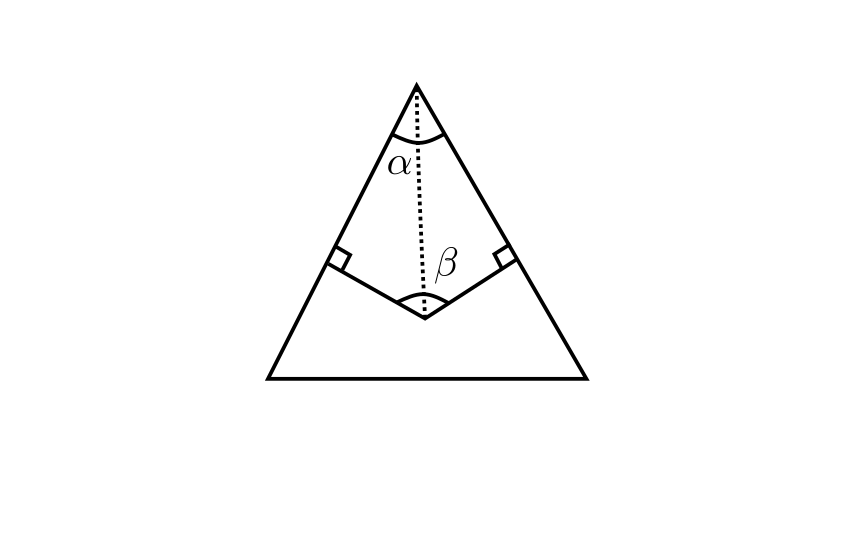
\includegraphics[width=.25\textwidth]{background/switch-angles}
\caption{The relationship between the angles incident to a vertex and
the interior angles of the area polygon on the sphere.}
\label{fig:switcheroo}
\end{figure}



This gives a  formula for computing the curvature at an interior vertex.
The \EMPH{angle defect} at a vertex $d(v)$ is the difference between $2\pi$ and
the sum of the incident angles.  Let $F_v$ denote the faces containing $v$  
and let $\alpha_f$  denote the interior  angle of face $f$ at $v$, then
\begin{equation} \label{eqn:defect}
d(v):=2\pi -\sum_{f\in F_v}\alpha_f.
\end{equation}
Since $\beta_i=\pi-\alpha_i$,
we can use our formula for the area of a polygon on the sphere,
\eqnref{sphere-area}, to compute the Gaussian curvature at $v$
by
$$K(v)=2\pi -n\pi+\sum_{i}^n \beta_i=2\pi-n\pi +\sum_{i}^n (\pi-\alpha_i) =2\pi-\sum_i^n\alpha_i=d(v)$$
 and the
 angle defect is equal to the discrete curvature in \defref{discrete-curvature-vertex}
 and in \eqnref{discrete-gaussian}.







Combining the above definitions  we have

\begin{theorem}[The Discrete Gauss-Bonnet Theorem] \label{thm:g-b-d}

If $S$ is a triangulated surface with  boundary $\partial S$ then

$$\sum_{v\in V_{int}} K(v) + \sum_{v\in V_{\partial S}} k_g(v) = 2\pi \chi(S)$$
where $K(v)$ is the discrete Gaussian curvature
of a vertex, $k_g(g)$ is the discrete geodesic curvature,  and
$\chi$ is the Euler characteristic.
\end{theorem}



